\documentclass[11pt]{report}
\usepackage{polski} %przydatne podczas składania dokumentów w j. polskim
\usepackage{setspace}
\usepackage[utf8]{inputenc} %kodowanie znaków, zależne od systemu
\usepackage[T1]{fontenc} %poprawne składanie polskich czcionek
\usepackage{subfigure}
\usepackage{psfrag}
\usepackage{tgheros}
\renewcommand{\familydefault}{\sfdefault}
%pakiety dodające dużo dodatkowych poleceń matematycznych
\usepackage{amsmath}
\usepackage{amsfonts}
%pakiety wspomagające i poprawiające składanie tabel
\usepackage{supertabular}
\usepackage{array}
\usepackage{tabularx}
\usepackage{hhline}
\usepackage{float}
\usepackage{indentfirst}
\usepackage{color}
\usepackage{enumerate}
\usepackage[a4paper, total={6in, 10in}]{geometry}
\usepackage{etoolbox}
\makeatletter
\patchcmd{\chapter}{\if@openright\cleardoublepage\else\clearpage\fi}{}{}{}
\makeatother
\usepackage{titlesec} 
\usepackage{graphicx}

%definicje własnych poleceń
\newcommand{\R}{I\!\!R} %symbol liczb rzeczywistych, działa tylko w trybie matematycznym
\newtheorem{theorem}{Twierdzenie}[section] %nowe otoczenie do składania twierdzeń

\newcommand*{\fancychapterstyle}{%
\titleformat{\chapter}{\bfseries\huge}{\filright}{1ex}
{\thechapter . }
}

%tutaj zaczyna się właściwa treść dokumentu
\begin{document}
	\bibliographystyle{unsrt} %tylko gdy używamy BibTeXa, ustawia polski styl bibliografii
	\clearpage
\thispagestyle{empty}

\setstretch{2}
\begin{center}
	\vspace*{2cm}
	\textbf{{\Huge ZASTOSOWANIE INFORMATYKI W~MEDYCYNIE}}
	
	\vspace{0.8cm}	
	\textbf{{\Huge PROJEKT}}
	
	\vspace{1.6cm}	
	\textbf{{\huge TEMAT:\textit{ Detekcja zespołu QRS w sygnale EKG}}}
	
	\vspace{1.2cm}	
	\textbf{{\LARGE PROWADZĄCY:}}
	
	\vspace{0.1cm}	
	\textbf{{\LARGE dr hab. inż. Robert Burduk}}
\end{center}

\begin{flushright}
	\vspace{7cm}
	\textbf{{\LARGE AUTOR:}}
	
	\vspace{0.1cm}	
	\textbf{{\LARGE Radosław Taborski 209347}}
\end{flushright}

	
	\tableofcontents %spis treści
	\newpage
	\fancychapterstyle
	\chapter{Cel projektu}
	Celem projektu jest stworzenia aplikacji, która ma analizować sygnał EKG pod kątem obecności w nim zespołu QRS. Aplikacja automatycznie wykrywa początki oraz końce zespołów, a także załamki: Q, R oraz S. 
	
	Właściwa analiza sygnału EKG, a w tym i zespołów QRS, ułatwia wykrywanie chorób mięśnia sercowego, dlatego bardzo istotne jest komputerowe wspomaganie tejże analizy. Wspomaganie takie może w znacznym stopniu przyspieszyć diagnozowanie chorób i zwracać uwagę lekarza na ewentualne nieprawidłowości.
	
	\chapter{Funkcjonalność aplikacji}
	W stworzonej aplikacji dostępne są następujące funkcje użytkowe:
	\begin{itemize}
		\item wczytanie pliku txt z sygnałem EKG;
		\item detekcja zespołów QRS w sygnale EKG;
		\item detekcja załamków Q, R oraz S;
		\item wizualizacja sygnału wraz z zaznaczeniem wykrytych załamków;
		\item wypisanie charakterystycznych punktów w aplikacji;
		\item zapis wyników detekcji do pliku txt.
	\end{itemize}
	
	\chapter{Algorytm}
	W ramach projektu w stworzonej aplikacji został zaimplementowany algorytm wzorujący się na algorytmie stworzonym przez dwóch badaczy o nazwiskach: Pan oraz Tompkins~[\ref{bib:algorithm}], który charakteryzuje się poprawnością detekcji zespołów QRS na poziomie 99,3\% skuteczności. \newline
	
	Algorytm ten polega na początkowym odfiltrowaniu sygnału, po którym wykonany zostaje szereg operacji matematycznych mających na celu jednoznaczne określenie fragmentów sygnału które są zespołami QRS.
	
	Początkowy sygnał EKG schematycznie został pokazany na rysunku \ref{fig:EKG}, natomiast po przetworzeniu tego sygnału wg. algorytmu Pan-Tompkins odtrzymuje się sygnał zbliżony do tego ukazanego na rysunku \ref{fig:sig}.
	
	\begin{figure} [H]
		\centering
		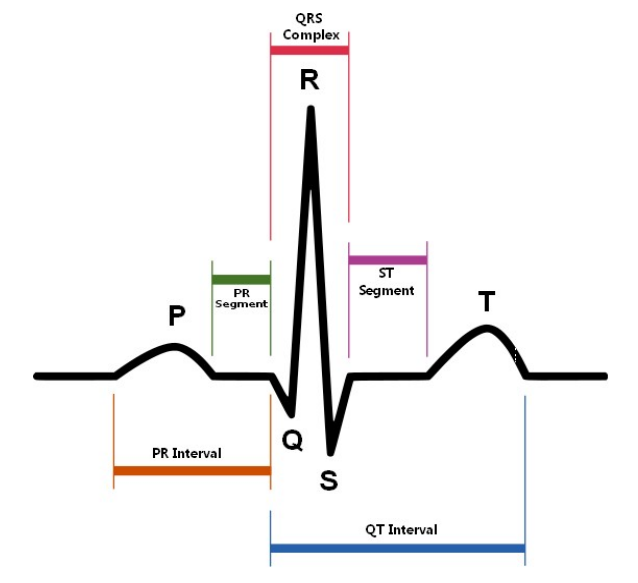
\includegraphics[width=0.5\linewidth]{EKG.png}
		\caption{Schematyczny kształt odcinka sygnału EKG}
		\label{fig:EKG}
	\end{figure}
	\vspace{2cm}
	
	\begin{figure} [H]
		\centering
		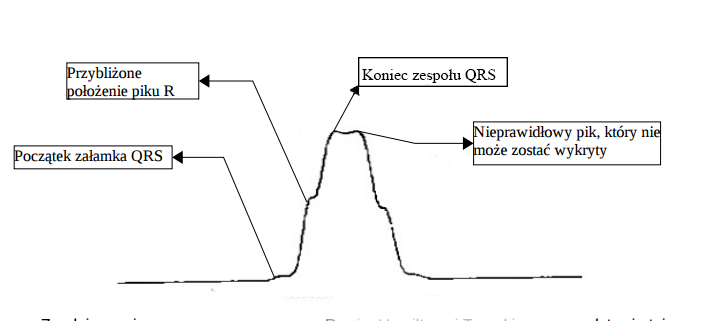
\includegraphics[width=0.8\linewidth]{sig.png}
		\caption{Sygnał na podstawie którego można podjąć decyzję o istnieniu zespołu QRS}
		\label{fig:sig}
	\end{figure}
	\vspace{2cm}
	
	Przetwarzanie sygnału polega na wykonaniu kolejno:
	\begin{itemize}
		\item przefiltrowanie sygnału filtrami górno i dolnoprzepustowymi, usuwając częstotliwości spoza przedziału 5-15Hz;
		\item wykonaniu operacji różnicowania na sygnale Równanie: $y[nT]=x[nT]-x[(n-1)T]$; 
		\item podniesieniu sygnału do kwadratu. Równanie: $y(nT)=[x(nT)]^2$;
		\item uśrednienie sygnału prostokątnym oknem czasowym f o długości 150ms i amplitudzie $\frac{1}{0.15*Fs}$. Równanie: $y[nT]=(x*f)[nT]$;
	\end{itemize}
	W powyższych wzorach: \newline
	x(nT)- n-ta próbka sygnału  poprzedzającego daną operację \newline
	y(nT)- n-ta próbka sygnału  wynikowego po danej operacji \newline
	Fs-częstotliwość sygnału EKG \newline
	
	Po wykonaniu powyższych kroków, długości zboczy rosnących w sygnale oznaczają długości odpowiadającym im zespołom QRS w sygnale wejściowym, a punkt przegięcia na tym zboczu przybliża położenie załamka R, tak jak zostało to pokazane na rysunku \ref{fig:sig}. Detekcja odpowiednich pików w sygnale nie jest możliwa przy pomocy lokalnych maksimów, ponieważ wykrywany zostaje również pik nieoznaczający końca zespołu QRS. Dlatego w algorytmie po wykryciu pierwszego piku, kolejny pik może zostać wykryty dopiero gdy sygnał osiągnie połowę wartości tego piku, czyli w  okolicy połowy zbocza malejącego.
	
	Powyższy algorytm nadaje się do badania sygnałów EKG w czasie rzeczywistym, jednak detekcja pojedynczego zespołu QRS zostaje zakończona dopiero w połowie zbocza opadającego przetworzonego sygnału, a więc detekcja następuje z opóźnieniem kilkudziesięciu ms.
	
	Dodatkowo po wykryciu pików wykrywa się również tzw. "znaki zaufania" we wstępnie przefiltrowanym sygnale jako maksymalne wartości w znalezionych przedziałach, a następnie odrzucić te które są mniejsze niż 5\% maksymalnego znalezionego znaku zaufania. Tak znalezione punkty są załamkami R.
	
	\chapter{Interfejs użytkownika}
	Aplikacja została wykonana w języku C\# w technologi WPF (ang. Windows Presentation Foundation), które z kolei opiera się na języku XML. Wykorzystanie tej technologii umożliwia tworzenie aplikacji okienkowych w postaci grafiki wektorowej.\newline
	
	Dostępne elementy:
	\begin{itemize}
		\item tabela z wynikami detekcji załamków Q, R i S;
		\item pole na wykres sygnału EKG, z podpisanymi osiami oraz skalowalną siatką;
		\item przyciski "+" oraz "-" umożliwiające rozciąganie oraz skurczenie wykresu w poziomie;
		\item pola tekstowe ze ścieżką wczytanego pliku oraz ze ścieżką pliku wynikowego;
		\item przyciski "Wczytaj" oraz "Zapisz" otwierające dodatkowe okno dialogowe do wyboru odpowiedniego pliku na dysku oraz wykonujące na tych plikach operacje, odpowiednio odczytanie danych oraz wpisanie danych;
		\item przycisk "Rysuj" umożliwiający wyświetlenie wczytanego wykresu EKG;
		\item przycisk "Detekcja" wykonujący szereg operacji na sygnale w celu odnalezienia zespołu QRS oraz załamków występujących w tym zespole.
	\end{itemize}
	
	\begin{figure} [H]
		\centering
		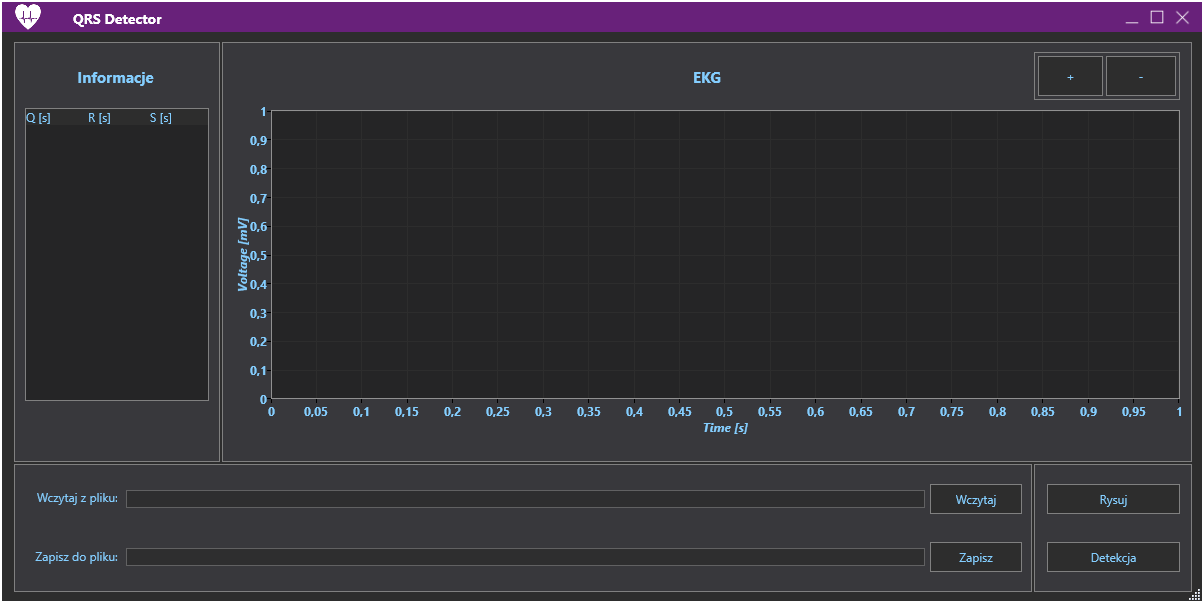
\includegraphics[width=1\linewidth]{GUI.png}
		\caption{Wygląd aplikacji po uruchomieniu}
		\label{fig:GUI}
	\end{figure}
	\vspace{2cm}

	\chapter{Prezentacja działania}
	Wybierając plik z dysku nie trzeba pamiętać pełnej ścieżki do pliku, a wystarczy znaleźć właściwy plik w otwartym oknie dialogowym. Analogicznie sytuacja wygląda podczas zapisu pliku wynikowego na dysku.
	
	\begin{figure} [H]
		\centering
		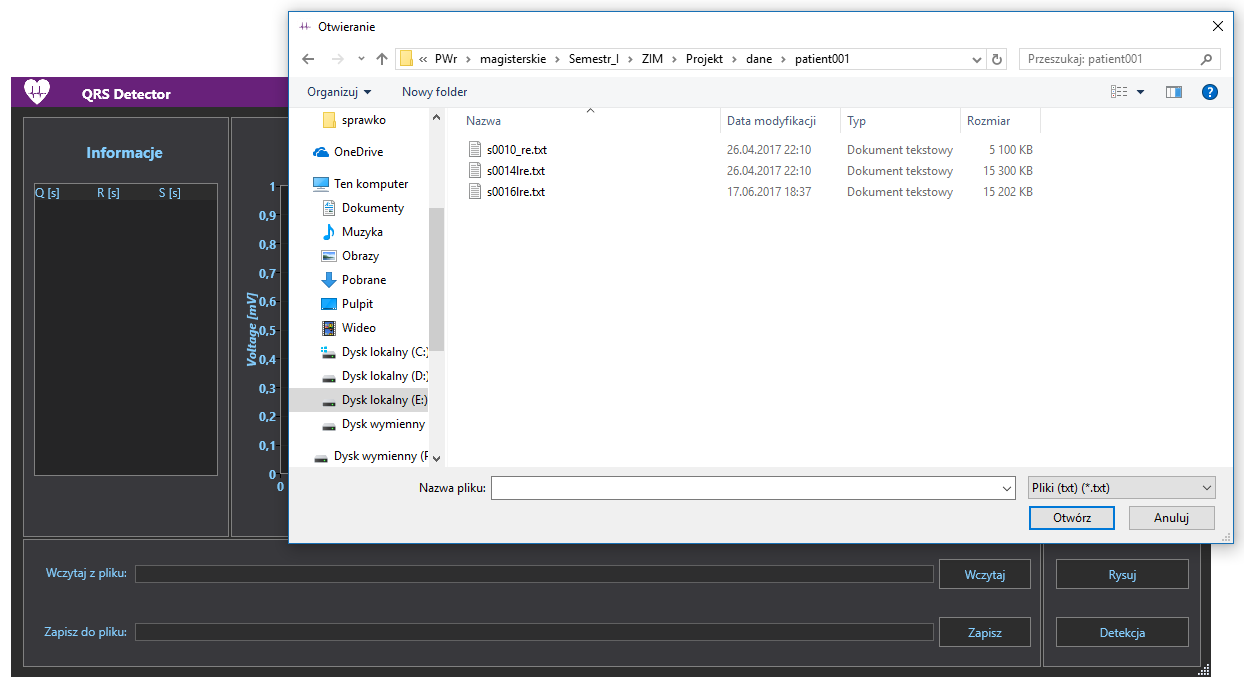
\includegraphics[width=1\linewidth]{okno_dialogowe.png}
		\caption{Wybór pliku z danymi}
		\label{fig:okno_dialogowe}
	\end{figure}
	\vspace{2cm}
	
	Dane wejściowe muszą być w formacie przedstawionym na rysunku \ref{fig:wejscie}. Gdzie pierwsza kolumna oznacza czas pomiaru konkretnej próbki podany w sekundach, a pozostałe kolumny oznaczają pomiary z piętnastu kanałów badania EKG. podane w miliwoltach. Dane sygnału EKG w takim formacie można pozyskać ze strony physionet.org postępując według poradnika umieszczonego na tej stronie [\ref{bib:physio}].
	\begin{figure} [H]
		\centering
		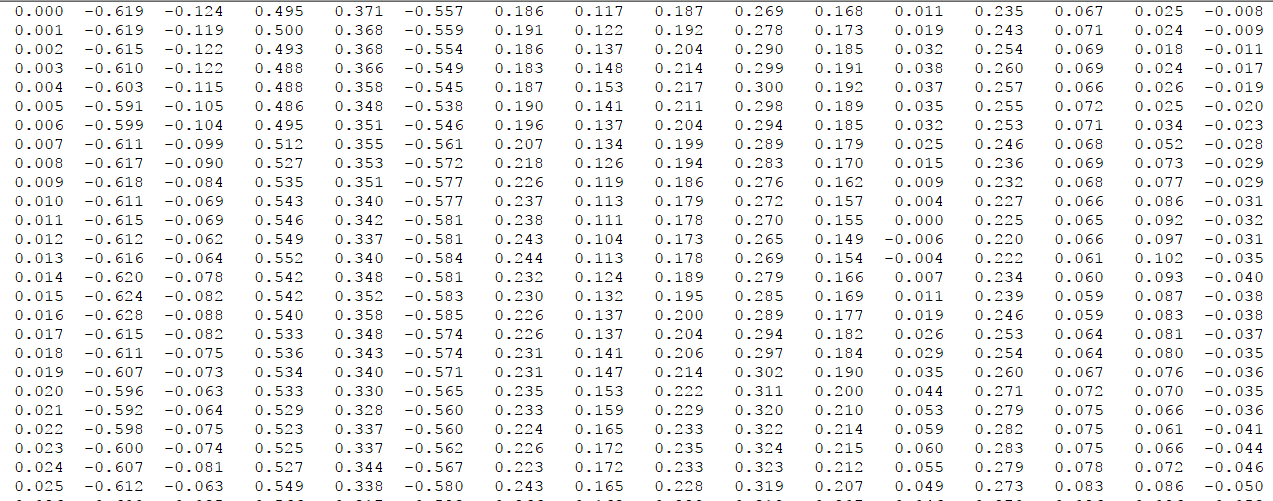
\includegraphics[width=1\linewidth]{wejscie.png}
		\caption{Zawartość pliku txt z przykładowymi danymi wejściowymi}
		\label{fig:wejscie}
	\end{figure}
	\vspace{2cm}

	Po wybraniu pliku z danymi mamy możliwość wyświetlenia badanego sygnału poprzez kliknięcie w przycisk "Rysuj", bądź też przeprowadzenia detekcji zespołów QRS bez wyświetlania sygnału. Druga opcja jest szczególnie użyteczna w sytuacji gdy użytkownikowi zależy wyłącznie na pliku wynikowym.
		
	\begin{figure} [H]
		\centering
		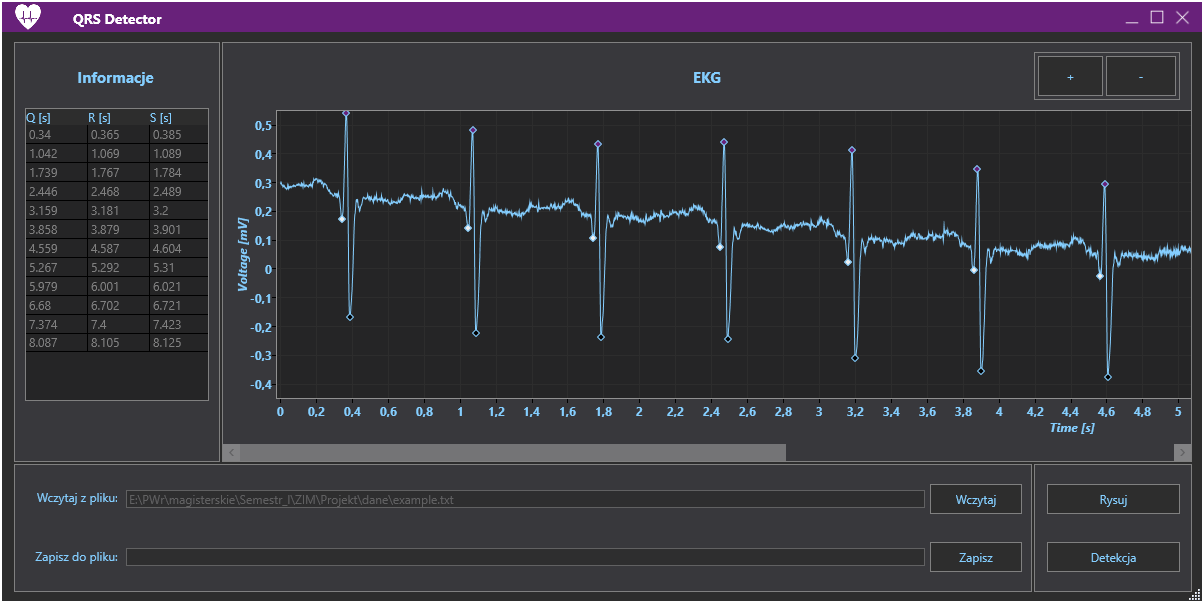
\includegraphics[width=1\linewidth]{wykres.png}
		\caption{Wyświetlony wykres wraz z wykrytymi załamkami Q, R oraz S}
		\label{fig:wykresy}
	\end{figure}
	\vspace{2cm}
	
	Klikając na przycisk "Zapisz" użytkownik ma możliwość utworzenia nowego pliku txt, bądź też nadpisania pliku już istniejącego. Do pliku tego zostają wpisane wyniki detekcji, które zaprezentowane zostały na rysunku \ref{fig:wynik}. Występujące w sygnale zespoły QRS zostały wypunktowane oraz dla każdego z punktów charakterystycznych zespołu QRS wypisane zostały jego parametry tj. czas wystąpienia podane w sekundach, oraz napięcie podane w miliwoltach.
	
	\begin{figure} [H]
		\centering
		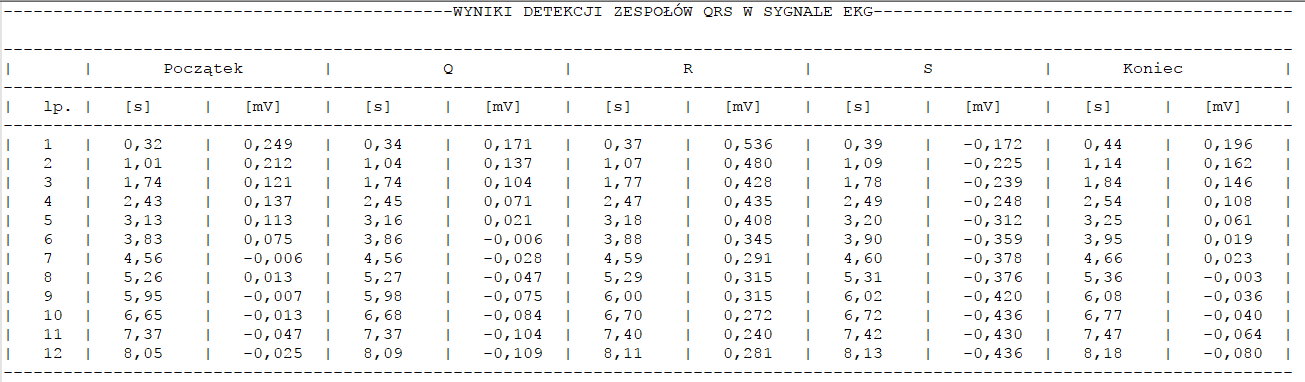
\includegraphics[width=1\linewidth]{wynik.png}
		\caption{Zawartość pliku txt z wynikami detekcji}
		\label{fig:wynik}
	\end{figure}
	\vspace{2cm}
	
	\chapter{Bibliografia}

\vspace*{1cm}

\begin{enumerate}[\lbrack 1\rbrack]
	\item http://www.robots.ox.ac.uk/~gari/teaching/cdt/A3/readings/ECG/Pan+Tompkins.pdf \label{bib:algorithm} \newline
	
	\item http://people.ece.cornell.edu/land/courses/ece5030/labs/s2013/QRS\_detect\_review.pdf \label{bib:method}
	
	\item http://physionet.org/tutorials/physiobank-text.shtml \label{bib:physio} \newline
	
\end{enumerate}


\end{document}
